% "{'chapitre':'slci_multiphy','classe':('PSI'),'type':('application'),'titre':'La Seine Musicale', 'source':'Concours Centrale - MP 2020','comp':['B2-02',],'corrige':True}"
\setchapterimage{fig_00.png}
\chapter*{Application \arabic{cptApplication} \\ La Seine Musicale -- \ifprof Corrigé \else Sujet \fi}
\addcontentsline{toc}{section}{Application \arabic{cptApplication} : La Seine Musicale  -- \ifprof Corrigé \else Sujet \fi}
\setcounter{question}{0}
\iflivret \stepcounter{cptApplication} \else
\ifprof  \stepcounter{cptApplication} \else \fi
\fi

\marginnote{Concours Centrale -- MP 2020}
\marginnote{\UPSTIcompetence[2]{B2-02}}
\begin{marginfigure}
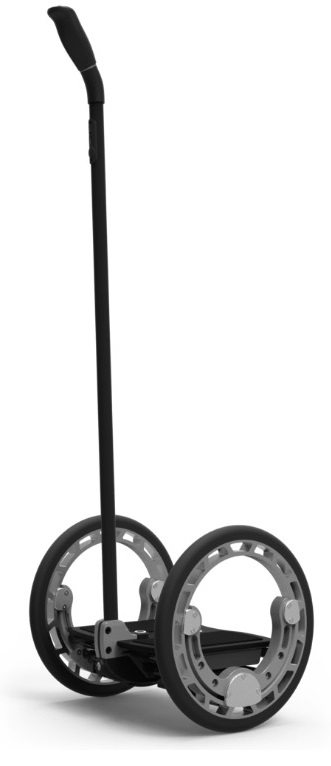
\includegraphics[width=\linewidth]{fig_01}
\end{marginfigure}

\ifprof
\else
La Seine Musicale est un équipement à vocation musicale à fort rayonnement culturel, dont l’objet est de créer
ou d’aménager des espaces pour des concerts, des expositions, des installations permanentes ou provisoires.

L’un des défis architecturaux de ce projet consiste à mettre en mouvement la voile, %(\autoref{fig_01}), 
équipée de 470 panneaux photovoltaïques, autour de l’auditorium, tout en garantissant une acoustique exceptionnelle.

\begin{marginfigure}
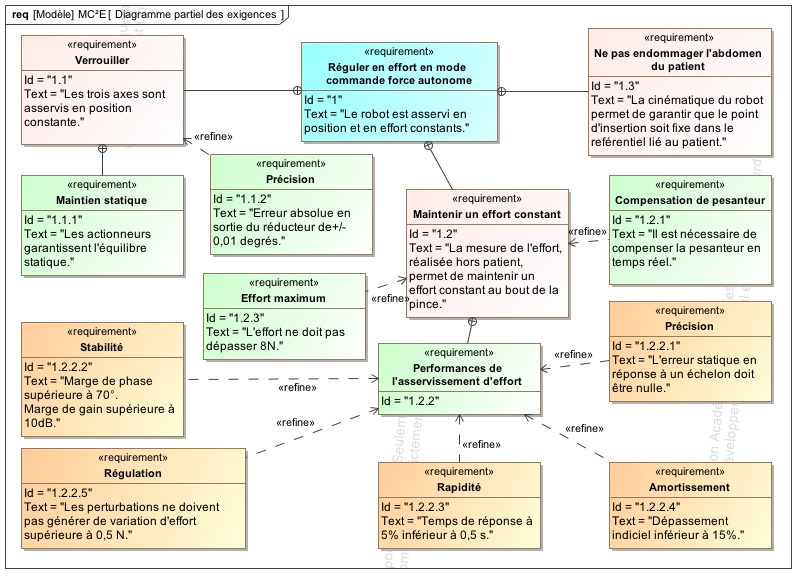
\includegraphics[width=\linewidth]{fig_05}
\caption{Schéma d’architecture de la voile solaire \label{fig_05}}
\end{marginfigure}

Les deux demi-voiles sont mises en mouvement de manière indépendante par des chariots motorisés, ainsi qu’une couronne motorisée déplaçant chacun des sommets des demi-voiles par l’intermédiaire
de bielles. 

Chaque chariot (central et latéral) se déplace grâce à quatre galets, appelés galets de roulement, qui roulent
sur les deux rails circulaires concentriques de la voie médiane de roulement et grâce à quatre autres galets de
guidage qui roulent sur les côtés des deux rails. Chacun des deux chariots centraux est motorisé à l’aide de deux
motoréducteurs qui entraînent chacun en rotation deux des quatre galets de roulement.
Afin d’optimiser son rendement énergétique, cette voile se déplace chaque jour toutes les 15 minutes pour suivre
le soleil du garage Est au garage Ouest.% à la vitesse angulaire maximale de \SI{0,18}{\degres.s^{-1}}.

Afin d’effectuer un premier dimensionnement en phase d’avant-projet des solutions
techniques choisies, un modèle multiphysique simple de la chaîne de traction d’un chariot motorisé est réalisé
(\autoref{fig_08}).
\textbf{On se place dans le cas le plus défavorable avec un seul motoréducteur fonctionnel qui entraîne
deux galets de roulement (roue).}


\begin{figure}[H]
\centering
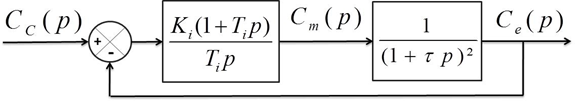
\includegraphics[width=\linewidth]{fig_08}
\caption{Modèle multiphysique du déplacement d’une demi-voile \label{fig_08}}
\end{figure}

Le modèle multiphysique est constitué de trois parties :
\begin{itemize}
\item commande en tension qui résulte de la superposition de deux rampes pour générer la loi de vitesse trapézoïdale;
\item modèle électrique constitué d’un moteur à courant continu alimenté;% (courant nominal de \SI{10,5}{A}) par une source de tension idéale (\SI{550}{V}) ;
\item modèle mécanique constitué d’un réducteur, d’une roue de chariot, d’une masse mobile de la demi-voile et
d’un capteur de position.
\end{itemize}
%Une première simulation est présentée \autoref{fig_09}. On appelle déplacement du chariot gauche par rapport au sol
%le déplacement du point $C_G$  par rapport à $\rep{g}$. On rappelle $\vect{OC_G}=R\vect{y_{C_G}}$ avec $R=\SI{22,750}{m}$.


%\subparagraph{\label{q4}}\textit{À partir des courbes \autoref{fig_09}, conclure quant au respect des exigences Id 1.1 et Id 1.2.}
%\ifprof
%\begin{corrige}
%
%\end{corrige}
%\else
%\fi

Lors de son déplacement, il peut arriver que la voile soit soumise à l’effet du vent. Il est donc important de
le prendre en compte dans le modèle pour évaluer son impact sur le déplacement. Par ailleurs, afin d’assurer
une durée de vie du moteur conforme à son mode de fonctionnement, il est important de pouvoir estimer la
consommation électrique du moteur en fonctionnement.

Le modèle \autoref{fig_08} a donc été enrichi de nouveaux blocs, à savoir : un capteur de courant, un capteur de tension
et l’effort extérieur lié au vent (échelon).
\fi


\question{\label{q5}}\textit{Sur la figure suivante, compléter les liens du modèle proposé pour prendre en compte
les deux capteurs.}
\ifprof
\begin{corrige}
\begin{figure}[H]
\centering
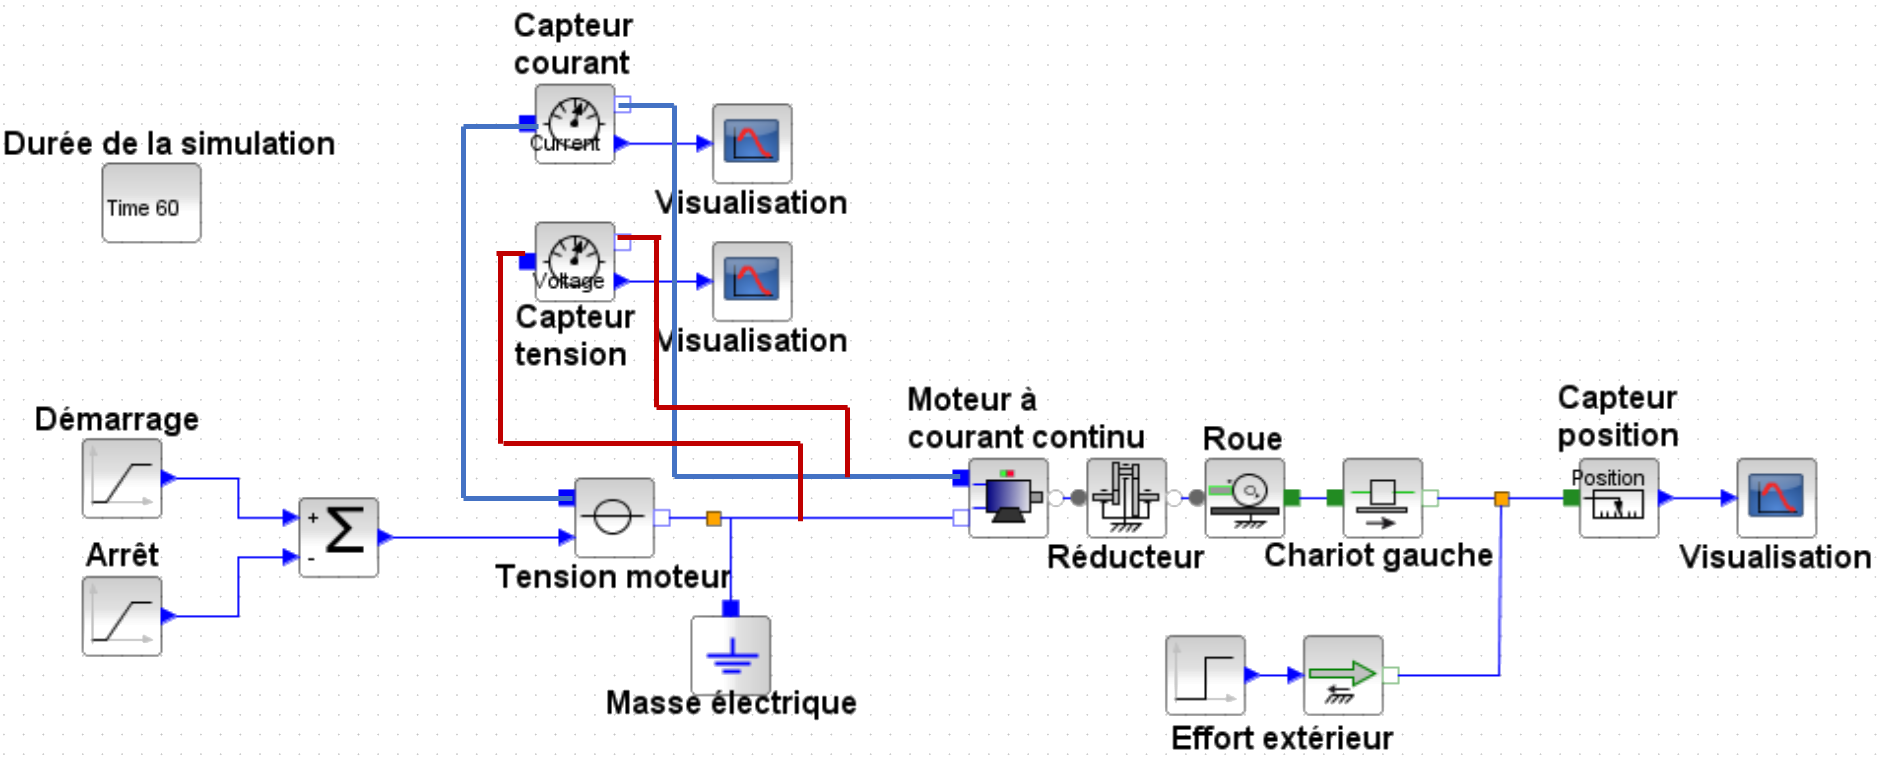
\includegraphics[width=\linewidth]{cor_1}
\end{figure}
\end{corrige}
\else
\fi

\ifprof
\else
\begin{figure}[H]
\centering
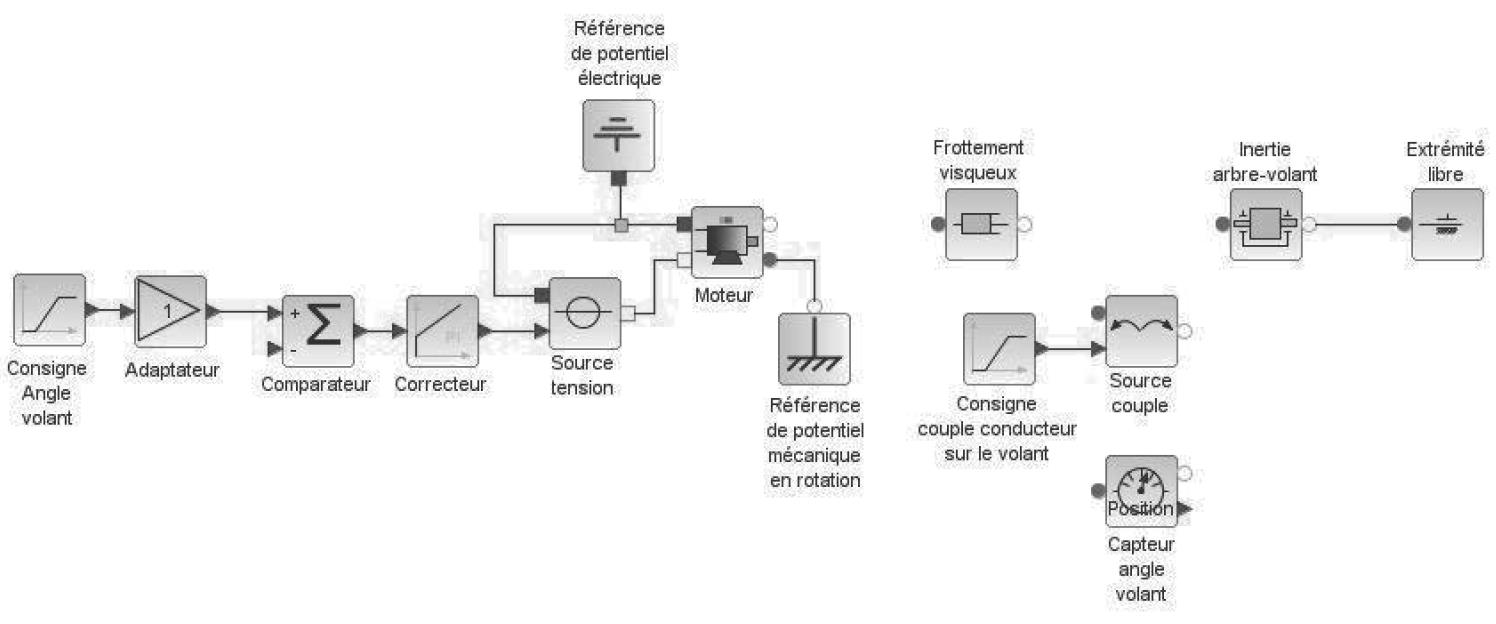
\includegraphics[width=\linewidth]{dr_01}
\caption{Modèle multiphysique du déplacement d’une demi-voile \label{dr_01}}
\end{figure}

\fi


\ifprof
\else
\begin{marginfigure}
\centering

\includegraphics[width=3cm]{Cy_01_Ch_01_Application_02_qr}
\end{marginfigure}
\fi